\cyanheader
\begin{frame}[fragile]{1D: En uendelig rekke}

\medskip
\textbf{a)} Hva slags rekke er dette? \\
\[
\sum_{n=1}^{\infty} \frac{1}{2^{n}} \;=\; \frac{1}{2}+\frac{1}{4}+\frac{1}{8}+\frac{1}{16}+\cdots
\]
\end{frame}

\cyanheader
\begin{frame}[fragile]{1D: En uendelig rekke}


\textbf{a)} Hva slags rekke er dette? \\
\[
\sum_{n=1}^{\infty} \frac{1}{2^{n}} \;=\; \frac{1}{2}+\frac{1}{4}+\frac{1}{8}+\frac{1}{16}+\cdots
\]

\medskip
Geometrisk rekke 
\[
\sum_{n=1}^{\infty} a_1 k^{n-1}
\]
med startledd $a_1=\tfrac12$ og kvotient $k=\tfrac12$.
\[\sum_{n=1}^{\infty} \frac{1}{2}\left(\frac{1}{2}\right)^{n-1}=\frac{1}{2}+\frac{1}{4}+\frac{1}{8}+\frac{1}{16}+\cdots\]
\end{frame}

\cyanheader
\begin{frame}[fragile]{1D: En uendelig rekke}


\textbf{b)} Finn et uttrykk for den n-te delsummen $s_n$, det vil si summen av de n første leddene. \\
\medskip

\[\sum_{n=1}^{\infty} \frac{1}{2}\left(\frac{1}{2}\right)^{n-1}=\frac{1}{2}+\frac{1}{4}+\frac{1}{8}+\frac{1}{16}+\cdots\]
\end{frame}

\cyanheader
\begin{frame}[fragile]{1D: En uendelig rekke}

\textbf{b)} Finn et uttrykk for den n-te delsummen $s_n$, det vil si summen av de n første leddene. 

\medskip
\begin{align*}
\sum_{n=1}^{\infty} \frac{1}{2}\left(\frac{1}{2}\right)^{n-1}&=\frac{1}{2}+\frac{1}{4}+\frac{1}{8}+\frac{1}{16}+\cdots\\
&=a_1\frac{k^n-1}{k-1}\\
&=\frac{1}{2}\frac{\left(\frac{1}{2}\right)^{n-1}-1}{\frac{1}{2}-1}\\
&=1-\left(\frac{1}{2}\right)^{n-1}
\end{align*}
\end{frame}


\cyanheader
\begin{frame}[fragile]{1D: En uendelig rekke}

\textbf{c)} Finnes det en grense for hvor stor delsummene kan bli?

\begin{columns}
\begin{column}{0.5\textwidth}
   \[
\frac{1}{2}+\frac{1}{4}+\frac{1}{8}+\frac{1}{16}+\cdots
\]
\end{column}

\begin{column}{0.5\textwidth}
\begin{figure}
    \centering
    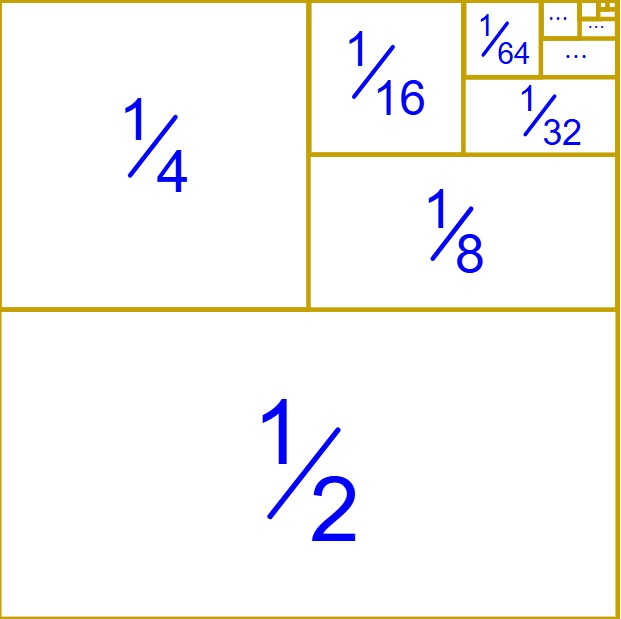
\includegraphics[width=0.8\linewidth]{R2K1D-3.png}
\end{figure}
\end{column}

\end{columns}

\end{frame}


\cyanheader
\begin{frame}[fragile]{1D: En uendelig rekke}

\textbf{d)} Lag et program du kan bruke til å regne ut $s_n$ for større og større $n$.\\

\end{frame}

\cyanheader
\begin{frame}[fragile]{1D: En uendelig rekke. (Bruker vanlig for-løkke)}
\begin{minted}[fontsize=\footnotesize]{python}
a1 = 0.5
k  = 0.5

liste_med_verdier_for_n = [1, 5, 10, 25, 50, 60]

minliste = [] # Tom liste som vi fyller med beregnede verdier

# Beregn verdiene én og én i en vanlig løkke
for n in liste_med_verdier_for_n:
    verdi = a1 * (k**n - 1) / (k - 1)
    minliste.append(verdi)

print(minliste)

# Skriv ut resultatene med tilhørende n
for i in range(len(minliste)):
    n = liste_med_verdier_for_n[i]
    verdi = minliste[i]
    print(f"s_{n} = {verdi}")

\end{minted}
\medskip
\end{frame}

\cyanheader
\begin{frame}[fragile]{1D:  Grafen til $s_n$ som funksjon av $n$}
\begin{figure}
    \centering
    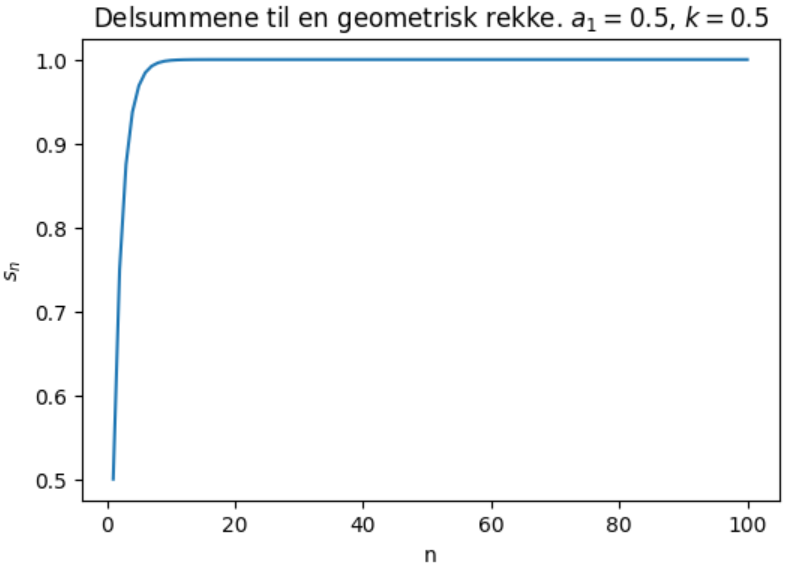
\includegraphics[width=0.7\linewidth]{R2K1D-2.png}
\end{figure}
\end{frame}

\cyanheader
\begin{frame}[fragile]{1D:  Grafen til $s_n$ som funksjon av $n$}
\begin{figure}
    \centering
    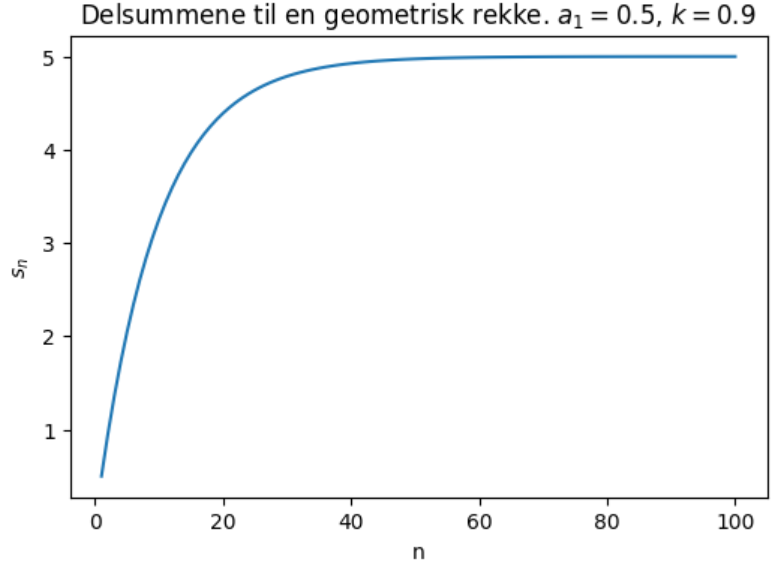
\includegraphics[width=0.7\linewidth]{R2K1D-4.png}
\end{figure}
\end{frame}

\cyanheader
\begin{frame}[fragile]{1D:  Grafen til $s_n$ som funksjon av $n$}
\begin{figure}
    \centering
    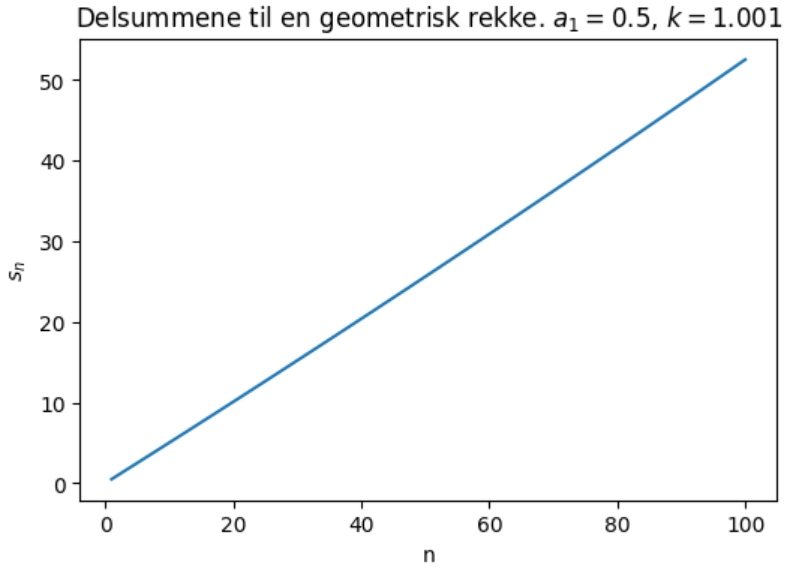
\includegraphics[width=0.7\linewidth]{R2K1D-5.png}
\end{figure}
\end{frame}

\cyanheader
\begin{frame}[fragile]{1D:  Grafen til $s_n$ som funksjon av $n$}
\begin{figure}
    \centering
    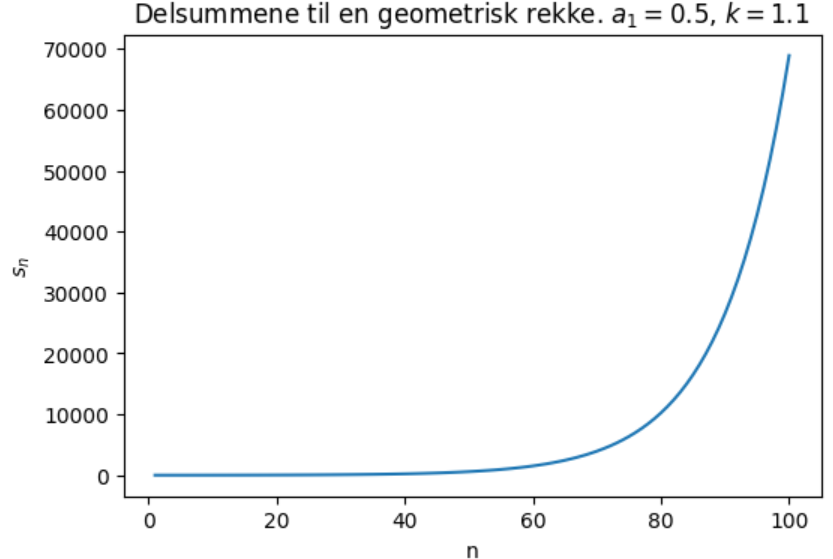
\includegraphics[width=0.7\linewidth]{R2K1D-6.png}
\end{figure}
\end{frame}

\blueheader
\begin{frame}{1D: Konvergent rekke}

\begin{blue*}{Definisjon}
La $s_n$ være summen av de $n$ første leddene i en uendelig rekke.  \\


Vi sier at den uendelige rekka \textbf{konvergerer} (er \emph{konvergent}) hvis uttrykket for $s_n$ har en grenseverdi $s$ når $n \to \infty$.  

\[
\lim_{n \to \infty} s_n = s
\]

Tallet $s$ kalles \emph{summen} av den uendelige rekka.  

\medskip
\textbf{Merk:} $s$ er en \emph{grenseverdi}, ikke en vanlig endelig sum slik som $s_n$.\\


Ordet \emph{konvergere} betyr å «nærme seg».
\end{blue*}
\end{frame}

\blueheader
\begin{frame}{1D: Divergent rekke}

\begin{blue*}{Definisjon}
Hvis en rekke ikke konvergerer, sier vi at den \textbf{divergerer} (er \emph{divergent}). \\


Ordet \emph{divergere} betyr å «fjerne seg».  

\medskip
\textbf{Eksempel:} Rekka
\[
\sum_{n=1}^{\infty} 2n = 2 + 4 + 6 + 8 + \cdots
\]
er divergent, siden $s_n \to \infty$ når $n \to \infty$.
\end{blue*}
\end{frame}

\redheader
\begin{frame}{1D: Konvergens av geometrisk rekke}


En uendelig geometrisk rekke med kvotient $k$ konvergerer når
\[
|k| < 1.
\]

Summen av den konvergente rekka er
\[
s = \frac{a_1}{1-k},
\]
der $a_1$ er det første leddet i rekka.

\vspace{1cm}
(Beviset står på side 60 i læreboka)

\end{frame}
\greenheader
\begin{frame}{1D: Eksempel}


Vi ser på den uendelige geometriske rekka med
\[
a_1 = \tfrac{1}{2}, \quad k = \tfrac{1}{2}.
\]

\medskip
Rekka blir
\[
\frac{1}{2} + \frac{1}{4} + \frac{1}{8} + \frac{1}{16} + \cdots
\]

Siden $|k| = \tfrac12 < 1$, konvergerer rekka. \\

Summen er
\[
s = \frac{a_1}{1-k} = \frac{\tfrac12}{1-\tfrac12} = 1.
\]

\end{frame}


\blueheader
\begin{frame}{1D: Sum av rekker i GeoGebra}
\centering
\begin{columns}
\begin{column}{0.4\textwidth}
I GeoGebra er kommandoene slik:\\
\vspace{1cm}
\texttt{Sum(0.5*0.5\textasciicircum(n-1),n,1,inf)}\\
\vspace{1cm}
\texttt{Sum(0.5*1.5\textasciicircum(n-1),n,1,inf)}
\end{column}

\begin{column}{0.6\textwidth}
\begin{figure}
    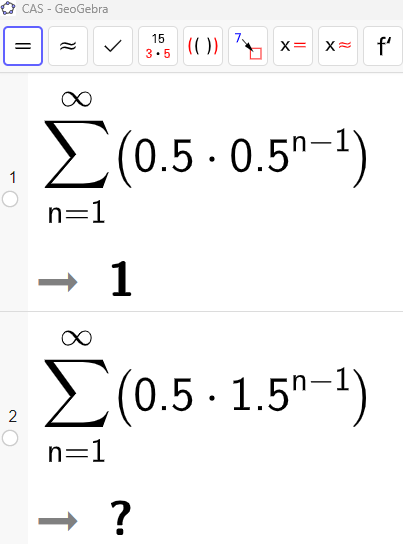
\includegraphics[width=0.6\linewidth]{R2K1D-7.png}
\end{figure}
\end{column}
\end{columns}
\end{frame}

\blueheader
\begin{frame}[fragile]{1D: Sum av rekker i Python med vanlig for-løkke}
\begin{minted}[fontsize=\normalsize]{python}
# Vi lager en tom liste som vi skal fylle med de 5 første partallene
minListe = []

# For-løkke: n går fra 1 til 5
for n in range(1, 6):
    tall = 2 * n       # regner ut partallet
    minListe.append(tall)     # legger tallet til i listen

print(minListe) # Output: [2, 4, 6, 8, 10]

# Regner ut summen av alle tallene i listen
summen = sum(minListe)
print(summen) # Output: 30

\end{minted}
\end{frame}



\blueheader
\begin{frame}[fragile]{1D: Sum av rekker i Python med \emph{list comprehension}}
\warn
\begin{minted}[fontsize=\Large]{python}
# Lager følgen av de 5 første partallene
f = [2*n for n in range(1,6)]
print(f)
# Output: [2, 4, 6, 8, 10]

# Regner ut summen av rekken
s = sum(f)
print(s)
# Output: 30
\end{minted}
\end{frame}




\redheader
\begin{frame}{1D: Geometrisk rekke med kvotient $k(x)$}

Når kvotienten til rekka er en funksjon av $x$, skriver vi $k(x)$ for kvotienten.  

\medskip
Summen av rekka vil da også variere med $x$, og vi skriver $s(x)$ for summen.  

\medskip
En uendelig geometrisk rekke
\[
\sum_{i=0}^{\infty} a \cdot k(x)^i \;=\; a + a\cdot k(x) + a\cdot k(x)^2 + a\cdot k(x)^3 + \cdots
\]
konvergerer når
\[
-1 < k(x) < 1.
\]

Summen av den konvergente rekka er gitt ved
\[
s(x) = \frac{a}{1-k(x)}.
\]

\medskip
For å finne \textbf{konvergensområdet} løser vi ulikheten
\[
-1 < k(x) < 1.
\]

\end{frame}

\greenheader
\begin{frame}{1D: Eksempel (a)}

En uendelig geometrisk rekke er gitt ved
\[
s(x) = 3 + 3(2x-1) + 3(2x-1)^2 + 3(2x-1)^3 + \cdots
\]

\textbf{a)} Bestem konvergensområdet til rekka.\\

\medskip
Kvotienten er 
\[
k(x) = 2x - 1.
\]

Vi løser
\[
-1 < k(x) < 1 \quad \Longrightarrow \quad -1 < 2x-1 < 1.
\]

\[
0 < x < 1.
\]

\textbf{Konvergensområdet er } $0 < x < 1$.
\end{frame}


\greenheader
\begin{frame}{1D: Eksempel (b)}
En uendelig geometrisk rekke er gitt ved
\[
s(x) = 3 + 3(2x-1) + 3(2x-1)^2 + 3(2x-1)^3 + \cdots
\]

\textbf{b)} Bestem $x$ slik at $s(x) = 3$.
Summen er
\[
s(x) =\frac{a_1}{1-k(x)}= \frac{3}{1-(2x-1)} = \frac{3}{2-2x}.
\]


Vi setter $s(x) = 3$:
\[
\frac{3}{2-2x} = 3 \quad \Longrightarrow \quad 2-2x = 1 \quad \Longrightarrow \quad x=\tfrac12.
\]

\textbf{Svar:} $x = \tfrac12$, som ligger i konvergensområdet $0<x<1$.
\end{frame}

\greenheader
\begin{frame}{1D: Eksempel (c)}
En uendelig geometrisk rekke er gitt ved
\[
s(x) = 3 + 3(2x-1) + 3(2x-1)^2 + 3(2x-1)^3 + \cdots
\]

\textbf{c)} Løs likningen $s(x) = 1$.\\

Vi setter $s(x) = 1$:
\[
\frac{3}{2-2x} = 1 \quad \Longrightarrow \quad 2-2x = 3 \quad \Longrightarrow \quad x = -\tfrac12.
\]

Men $x=-\tfrac12$ ligger \textbf{utenfor konvergensområdet} $0<x<1$.  

\medskip
\textbf{Svar:} Likningen $s(x)=1$ har ingen løsning.
\end{frame}

\blueheader
\begin{frame}{1D: Den harmoniske rekka}


Den harmoniske rekka divergerer
\[
\sum_{n=1}^{\infty} \frac{1}{n} \;=\; 1 + \tfrac{1}{2} + \tfrac{1}{3} + \tfrac{1}{4} + \tfrac{1}{5} + \cdots
\]

\medskip
Sammenlign leddene med en annen rekke som åpenbart divergerer:
  \[
  \tfrac{1}{2} + \tfrac{1}{3} + \tfrac{1}{4} +\tfrac{1}{5} +\tfrac{1}{6} +\tfrac{1}{7} +\tfrac{1}{8}+... \; \geq \; \tfrac{1}{2}+\tfrac{1}{4}+\tfrac{1}{4}+\tfrac{1}{8}+\tfrac{1}{8}+\tfrac{1}{8}+\tfrac{1}{8}+...
  \]

\medskip
\textbf{Konklusjon:} Den harmoniske rekka er et eksempel på at det ikke er nok at leddene blir små for at rekka skal konvergere.
\end{frame}

\blueheader
\begin{frame}{1D: Alternerende rekker}
Hvis vi lar leddene i en rekke veksle mellom å ha positivt og negativt fortegn, har vi en \emph{alternerende} rekke.

\begin{green*}{Eksempel: Alternerende harmonisk rekke}
    Hvis vi veksler på fortegnene til den harmoniske rekka, vil vi få en konvergent rekke som har en sum
    \[
    \sum_{n=1}^{\infty}\frac{(-1)^{n-1}}{n}=1-\frac{1}{2}+\frac{1}{3}-\frac{1}{4}+...
    \]

    \medskip
    (Se side 67)
\end{green*}
\end{frame}

\cyanheader
\begin{frame}[t]{1D: Eulerkonstanten}
Lag et program som regner ut
\[
E_n = \left(1 + \frac{1}{2} + \frac{1}{3} + \frac{1}{4} + \cdots + \frac{1}{n}\right) - \ln(n).
\]

\medskip
Skriv ut tallene $E_n$ for $n = 1,2,\ldots,100$. Hva ser du?

\end{frame}

\cyanheader
\begin{frame}[fragile]{1D: Eulerkonstanten med vanlig for-løkke}
\begin{minted}[fontsize=\footnotesize]{python}
from pylab import *  # Importerer blant annet log (ln)

# Vi setter et stort tall som "øverste grense" for summen
n_maks = 1_000_000  

# Vi lager en tom liste som skal inneholde leddene i den harmoniske rekken
harmonisk_følge = []  

# Vi fyller listen med 1/n for n = 1, 2, ..., n_maks
for n in range(1, n_maks+1):
    harmonisk_følge.append(1/n)

# Vi regner ut summen av de n_maks første leddene i den harmoniske rekken
# og trekker fra ln(n_maks). Dette nærmer seg Eulers konstant

s_n_maks = sum(harmonisk_følge) - log(n_maks)

# Vi skriver ut resultatet (en tilnærming til Eulers konstant)
print(s_n_maks) # Output: 0.5772161649014613
\end{minted}
\end{frame}

\redheader
\begin{frame}{1D: Euler-konstanten}
\[
E_n = \left(1 + \frac{1}{2} + \frac{1}{3} + \cdots + \frac{1}{n}\right) - \ln(n).
\]

\medskip
Følgen $\{E_n\}$ har en grenseverdi når $n \to \infty$.\\
\[
\gamma = \lim_{n \to \infty} \left( \sum_{k=1}^n \frac{1}{k} - \ln(n) \right).
\]

\medskip
\begin{itemize}
  \item $\gamma \approx 0.57721\ldots$\\
  \item Må ikke forveksles med tallet $e \approx 2.718\ldots$\\
  \item Det er ukjent om $\gamma$ er rasjonalt eller irrasjonalt.\\
\end{itemize}
\end{frame}

\blueheader
\begin{frame}{1D: Potensrekker}
\begin{blue*}{Definisjon}
En \textbf{potensrekke} er en uendelig rekke på formen
\[
\sum_{n=0}^{\infty} a_n (x-c)^n,
\]
der $a_n$ er koeffisienter og $c$ er sentrum for rekka.
\end{blue*}
\begin{green*}{Eksempel: Rekka for eksponentialfunksjonen}
\[
e^x = \sum_{n=0}^{\infty} \frac{x^n}{n!}.
\]
   
\end{green*}


\end{frame}























